\documentclass[a4paper]{article}


\usepackage[T1]{fontenc}    
\usepackage[utf8]{inputenc} 
\usepackage{textcomp}      
\date{} 					
\author{}                   
\usepackage{geometry}		
\geometry{ left=2cm, right=2cm, top=2cm, bottom=4cm, bindingoffset=5mm}

\usepackage{listings}
\usepackage{color}
\usepackage{longtable}


\definecolor{eminence}{RGB}{108,48,130}
\definecolor{myblue}{RGB}{65,105,225}


\lstset{
	keywordstyle=\color{myblue},  
	numbers=left,  
	stringstyle=\color{mymauve},
	numberstyle=\tiny\color{mygray} ,    
	commentstyle=\fontsize{9}{13}\itshape\color{mygreen}
}

\lstset{literate=
	{á}{{\'a}}1 {é}{{\'e}}1 {í}{{\'i}}1 {ó}{{\'o}}1 {ú}{{\'u}}1
	{Á}{{\'A}}1 {É}{{\'E}}1 {Í}{{\'I}}1 {Ó}{{\'O}}1 {Ú}{{\'U}}1
	{à}{{\`a}}1 {è}{{\`e}}1 {ì}{{\`i}}1 {ò}{{\`o}}1 {ù}{{\`u}}1
	{À}{{\`A}}1 {È}{{\'E}}1 {Ì}{{\`I}}1 {Ò}{{\`O}}1 {Ù}{{\`U}}1
	{ä}{{\"a}}1 {ë}{{\"e}}1 {ï}{{\"i}}1 {ö}{{\"o}}1 {ü}{{\"u}}1
	{Ä}{{\"A}}1 {Ë}{{\"E}}1 {Ï}{{\"I}}1 {Ö}{{\"O}}1 {Ü}{{\"U}}1
	{â}{{\^a}}1 {ê}{{\^e}}1 {î}{{\^i}}1 {ô}{{\^o}}1 {û}{{\^u}}1
	{Â}{{\^A}}1 {Ê}{{\^E}}1 {Î}{{\^I}}1 {Ô}{{\^O}}1 {Û}{{\^U}}1
	{œ}{{\oe}}1 {Œ}{{\OE}}1 {æ}{{\ae}}1 {Æ}{{\AE}}1 %{ß}{{\ss}}1
	{ű}{{\H{u}}}1 {Ű}{{\H{U}}}1 {ő}{{\H{o}}}1 {Ő}{{\H{O}}}1
	{ç}{{\c c}}1 {Ç}{{\c C}}1 {ø}{{\o}}1 {å}{{\r a}}1 {Å}{{\r A}}1
}


\usepackage{graphicx}
\usepackage{xcolor}
\usepackage{hyperref} 
\usepackage{fancyhdr}
\usepackage{amsmath}											
\pagestyle{fancy}
\fancyhf{}
\fancyhead[R]{2973140 - Felix Bühler  \\ 2893121 - Jan Leusmann \\  3141241 - Jamie Ullerich}
\fancyhead[L]{Scientific Visualisation \\ Sommersemester 2019 }
\renewcommand{\headrulewidth}{0.5pt} 				

\title{Exercise 10}

\begin{document}

\maketitle 
\thispagestyle{fancy}


\section*{Exercise 10. 1
Pre- and Post-Classification}

\section*{Exercise 10. 2
Composition Schemes in Direct Volume Rendering}

\begin{figure}[!ht]
	\centering
	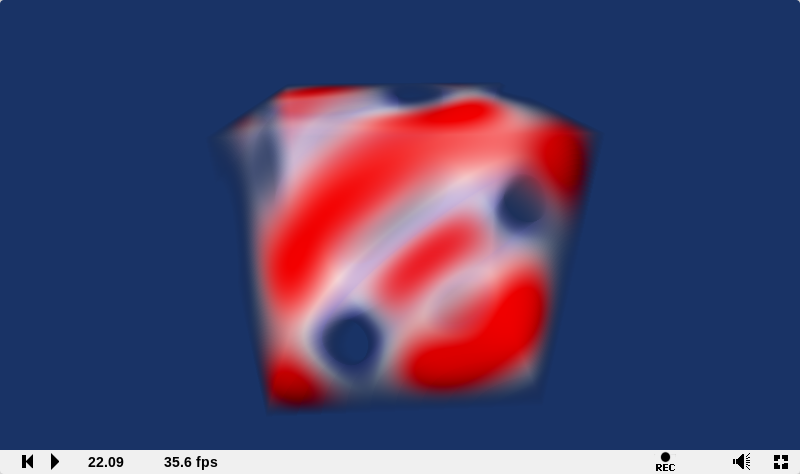
\includegraphics[width=0.7\linewidth]{1}
	\caption{Accumulation}
	\label{fig:1}
\end{figure}

\begin{figure}[!ht]
	\centering
	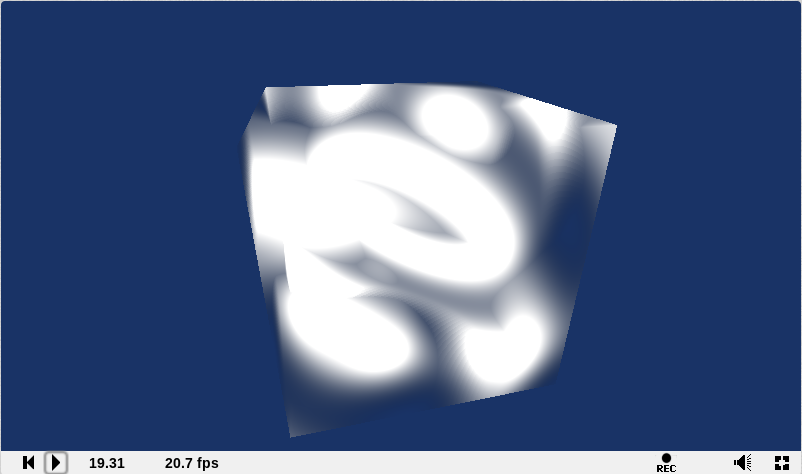
\includegraphics[width=0.7\linewidth]{2}
	\caption{Max. intensity projection}
	\label{fig:2}
\end{figure}

\begin{figure}[!ht]
	\centering
	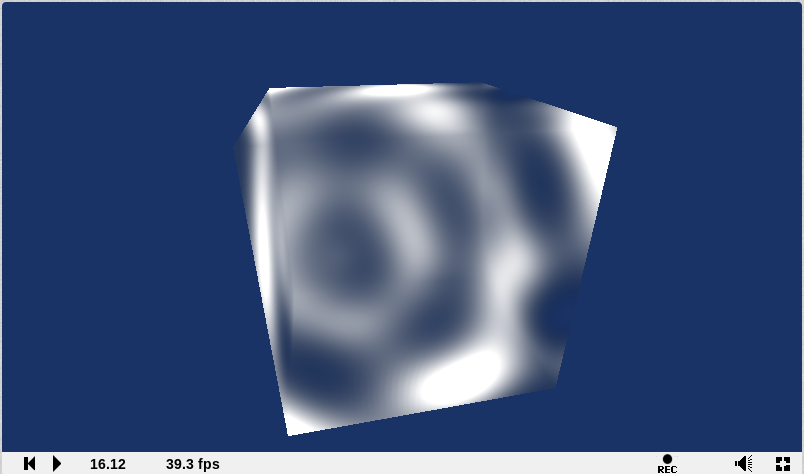
\includegraphics[width=0.7\linewidth]{3}
	\caption{Average intensity}
	\label{fig:3}
\end{figure}

\end{document}